\documentclass[a4paper,12pt]{article}
\usepackage[a4paper]{geometry}
\usepackage{color, hyperref}
\usepackage[hypcap]{caption}
\usepackage[utf8]{inputenc}
\usepackage{float}
\usepackage{array}
\usepackage{ulem}
\usepackage{contour}
\usepackage{listings}
\usepackage{booktabs}
\usepackage{multirow}
\usepackage{wrapfig, graphicx}
\usepackage{tikz}

\graphicspath{{./img}}
\hypersetup{
	colorlinks=true,
	breaklinks=true,
	linkcolor=black,
	pdftitle={PolyMessages - Sprint 2}
}

\definecolor{codegreen}{rgb}{0,0.6,0}
\definecolor{codegray}{rgb}{0.5,0.5,0.5}
\definecolor{codepurple}{rgb}{0.58,0,0.82}
\definecolor{backcolour}{rgb}{0.9,0.9,0.9}
\lstdefinestyle{myStyle}{
	backgroundcolor=\color{backcolour},
	commentstyle=\color{codegreen},
	keywordstyle=\color{magenta},
	numberstyle=\tiny\color{codegray},
	stringstyle=\color{codepurple},
	basicstyle=\ttfamily\footnotesize,
	breakatwhitespace=false,
	breaklines=true,
	captionpos=b,
	keepspaces=true,
	showspaces=false,
	showstringspaces=false,
	showtabs=false,
	tabsize=2,
	linewidth=0.95\linewidth,
	xleftmargin=0.2\linewidth,
	% padding=5px
}

\lstset{style=myStyle}


\renewcommand{\ULdepth}{1.8pt}
\contourlength{0.8pt}

\newcommand{\ul}[1]{%
	\uline{\phantom{#1}}%
	\llap{\contour{white}{#1}}%
}

\captionsetup{labelfont={it, bf}, textfont={it}}

\title{PolyMessages | Sprint 2}
\author{Eri Agnese, Marvin Bontemps, Lucas Nouguier}
\date{01 Mai 2022}

\begin{document}
\maketitle
\tableofcontents
\clearpage
\hypersetup{linkcolor=red}

\newgeometry{left=2cm,right=2cm,bottom=2cm, top=1.5cm}

\section{Protocole de communication}
\begin{figure}[h]
	\centering
	\hrulefill\\
	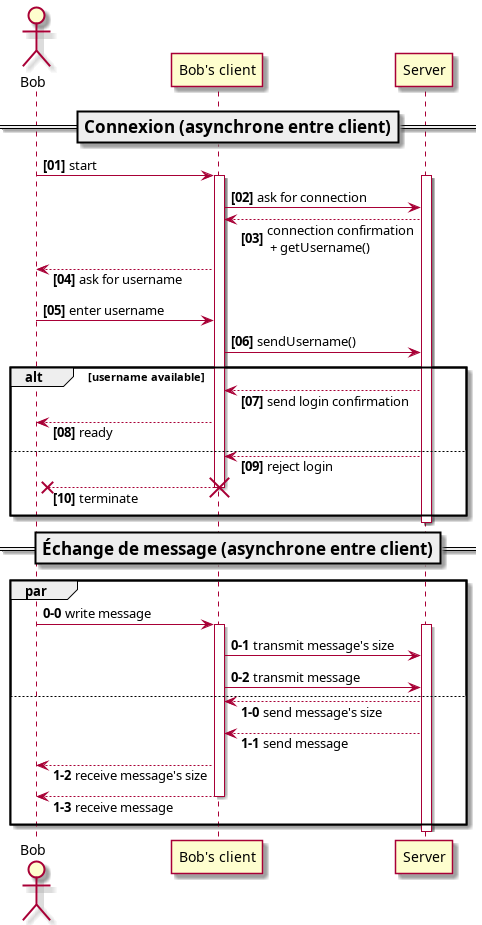
\includegraphics[width=0.45\linewidth]{sequence.png}
	\hfill
	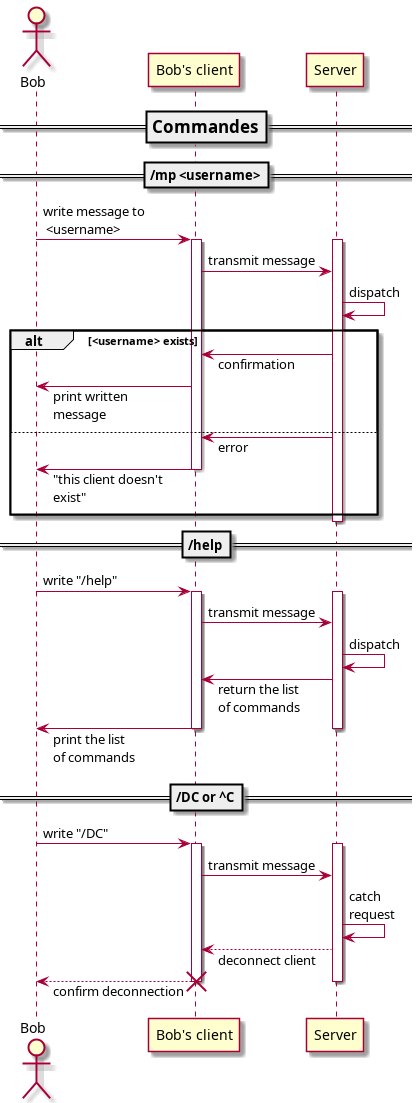
\includegraphics[width=0.4\linewidth]{commands.png}
	\caption{Protocole de communication clients/serveur}
	\hrulefill
\end{figure}

\pagebreak
\section{Architecture}
\begin{figure}[h]
	\centering
	\hrulefill\\
	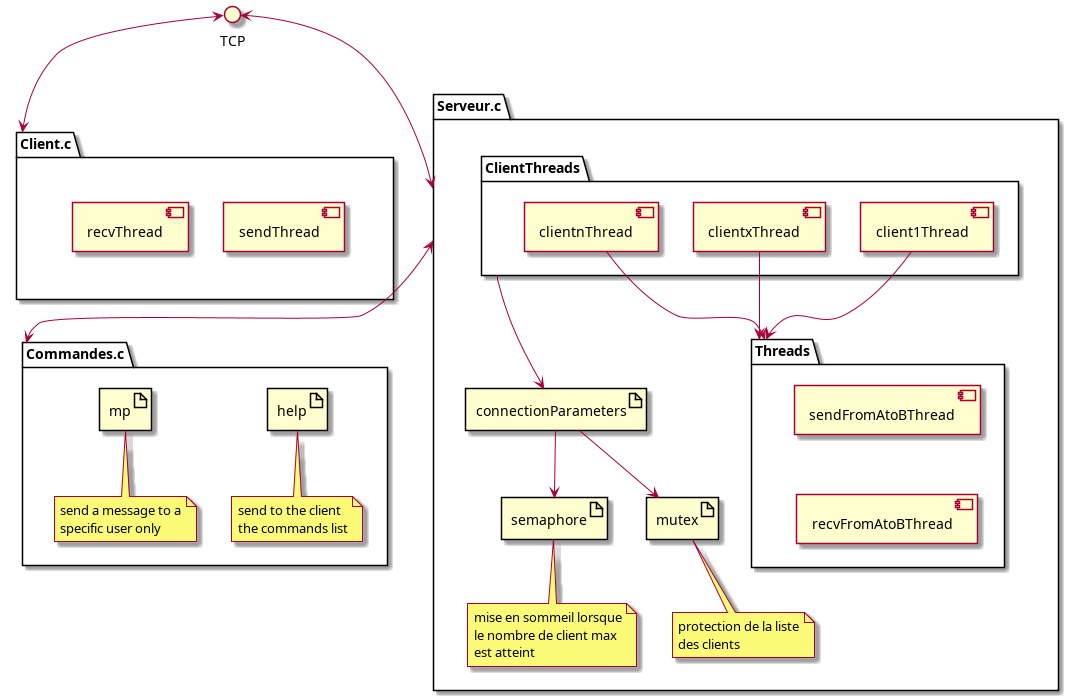
\includegraphics[width=\linewidth]{architecture.png}
	\caption{Architecture de la messagerie}
	\hrulefill
\end{figure}
\section{Répartition du travail}
\begin{wraptable}{r}{0.5\linewidth}
	\vspace{-0.5cm}
	\begin{tabular}{cccc}
		\toprule
		\multirow{2}{*}{Tâches} & \multicolumn{3}{c}{Étudiants}\\
		\cmidrule{2-4}
		& Lucas & Éri & Marvin\\
		\midrule
		Mutliclient & X\\
		\midrule
		MP & & & X\\
		\midrule
		Help & & X &X\\
		\midrule
		Protection des données & & X\\
		\bottomrule
	\end{tabular}
	\caption{Tâche effecutée par étudiant}
	\label{table:repartition}
	% \vspace{-1.5cm}
\end{wraptable}
La 2\textsuperscript{ème} version de la messagerie consistait à avoir une gestion multiclient. Il fallait pouvoir gérer la connexion/deconnexion de chaque client indépendamment des autres clients. Comme il y avait plusieurs clients, on a dû créer des variables globales qu'il a fallu protéger via des \textit{mutex} et \textit{sémaphores}. Une fonctionnalité de message privée entre 2 utilisateurs a également été mise en place (voir \ul{Table.~\ref{table:repartition}} \& \ul{Fig.~\ref{fig:gantt}}). Cette fois-ci, l'ensemble des fonctionnalités a été développé en asynchrone.

\begin{figure}[h]
	\centering
	\hrulefill\\
	\vspace{0.4cm}
	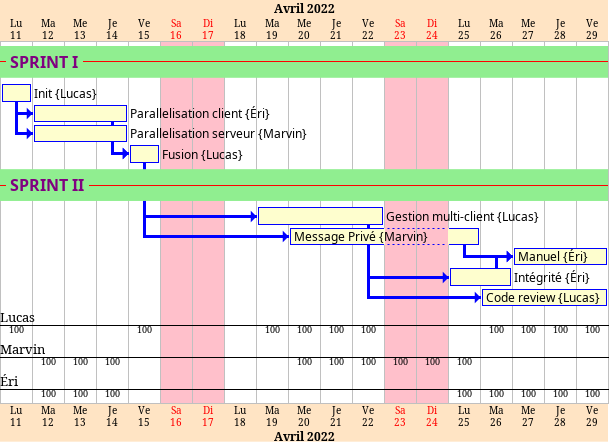
\includegraphics[width=\linewidth]{gantt.png}\\
	\caption{Diagramme de Gantt sur la réalisation du projet}
	\label{fig:gantt}
	\hrulefill
\end{figure}
\pagebreak
\section{Exécution du code}
Pour lancer la messagerie, il faut commencer par compiler et lancer le serveur
\begin{figure}[h]
	\centering
	\vspace{-0.1cm}
	\begin{lstlisting}[language=bash, gobble=4]
		[lucas@xps-lucas ~]$ gcc -o server serveur.c commandes.c
		[lucas@xps-lucas ~]$ ./server <PORT>
	\end{lstlisting}
\end{figure}

\noindent On peut alors lancer les clients
\begin{figure}[h]
	\centering
	\vspace{-0.2cm}
	\begin{lstlisting}[language=bash, gobble=4]
		[lucas@xps-lucas ~]$ gcc -o client client.c
		[lucas@xps-lucas ~]$ ./client <IP> <PORT>
	\end{lstlisting}
\end{figure}
\section{Difficultés}
\begin{itemize}
	\item Changement des structures de données pour les rendre plus facile d'utilisation \& de compréhension
	\item Fin des threads résolus via un \textit{exit(0)} lorsqu'un \textit{receive()} recevait une chaîne particulière
\end{itemize}
\end{document}